%%
%% AI-Assisted Experimentation Consulting for Educational Platform Adoption
%% ACM acmart manuscript LaTeX source.
%%

%% Force one-sided geometry to avoid mirrored page margins in manuscript mode.
\PassOptionsToPackage{twoside=false}{geometry}
\documentclass[manuscript,screen]{acmart}

%% Disable ACM copyright/reference footer blocks for draft submission.
\settopmatter{printacmref=false}
\setcopyright{none}
\renewcommand\footnotetextcopyrightpermission[1]{}

\AtBeginDocument{%
  \providecommand\BibTeX{{%
    Bib\TeX}}}

\usepackage{tikz}
\usetikzlibrary{arrows.meta, positioning, fit, backgrounds, calc}

%% Camera-ready (after acceptance): replace \setcopyright{none} with the
%% assigned value and add \copyrightyear, \acmYear, \acmConference, \acmISBN,
%% \acmDOI using metadata supplied by ACM.

\begin{document}

\title{AI-Assisted Experimentation Consulting for Educational Platform Adoption}

%
%\author{Zack Lee}
%\email{zlee@carnegielearning.com}
%\affiliation{%
%  \institution{Carnegie Learning}
%  \department{Research Team}
%  \city{Pittsburgh}
%  \state{Pennsylvania}
%  \country{USA}
%}

%\author{April Murphy}
%\email{amurphy@carnegielearning.com}
%\affiliation{%
%  \institution{Carnegie Learning}
%  \department{Research Team}
%  \city{Pittsburgh}
%  \state{Pennsylvania}
%  \country{USA}
%}

\renewcommand{\shortauthors}{Lee and Murphy}

\begin{abstract}
Educational software teams that wish to run A/B tests within their applications often need more than access to experimentation tools: translating broad learning goals or product features into concrete experimental designs can require expert consultation over multiple sessions. This planning layer has emerged as a recurring topic when onboarding new applications to \href{https://www.upgradeplatform.org/}{UpGrade}, an A/B testing platform designed to support educational experimentation at scale. This paper describes a prototype of an AI-assisted experimentation consultant that guides users through a six-phase workflow, from gathering a description of the app through generating a report that describes testable hypotheses, outcome measures, implementation details, and how to set up the experiment in the UpGrade UI. The report can then be used as a shared artifact between researchers, developers, product managers, and other stakeholders. 
\end{abstract}

\ccsdesc[500]{Applied computing~Education~Interactive learning environments}
\ccsdesc[300]{Computing methodologies~Artificial intelligence~Natural language processing}
\ccsdesc[300]{Human-centered computing~Human computer interaction (HCI)~Interactive systems and tools}

\keywords{AI-assisted experimentation, educational A/B testing, hypothesis refinement, human-in-the-loop AI, experiment planning, UpGrade}

\maketitle

\section{Introduction}

Adopting an educational A/B testing platform is rarely just about tool access. EdTech teams that want to run experiments in their own learning applications often need substantial expert consultation before they ever open the platform's interface. This can take the form of help deciding \emph{what} to experiment on, \emph{where} condition assignment should occur, \emph{how} variants should be implemented, and \emph{which} outcomes would make the result interpretable and actionable. This pattern has been visible in recent work supporting EdTech teams as they integrate with and onboard to \href{https://www.upgradeplatform.org/}{UpGrade}, an open-source A/B testing platform developed by \href{https://carnegielearning.com/}{Carnegie Learning}~\cite{upgrade} that is designed to address the specific constraints of embedding experiments in digital learning platforms used in real classrooms. As adoption expands to additional teams, recurring questions have arisen around topics such as where in the app the experiment should occur, condition assignment and consistency, outcome metrics, and client-side API instrumentation. While UpGrade's UI makes setting up, deploying, and managing experiments or feature flags simple, the challenge is often turning an idea--whether it maps to a product feature or how to convert a traditional experimental design to a digital learning environment--into a concrete plan to implement and deploy in UpGrade. This broader motivation extends beyond UpGrade: educational platforms have embedded randomized experiments, including \emph{in vivo} educational experiments, into everyday learning environments, suggesting a need for tools that help teams translate ideas into implementable experiment plans~\cite{williams2015inVivoEducationalExperiments}. 

This paper presents a prototype of an \textbf{AI-assisted experimentation consultant}, the \emph{AI Experiment Consultant}, designed to address this planning stage. The system is a web-based, chat-driven tool that guides users through a six-phase consulting workflow and produces a downloadable markdown report covering foundational concepts related to the client application, a refined hypothesis, a proposed UpGrade experiment design, a simulation summary, and implementation guidance. We illustrate this six-phase workflow with a fictional \emph{ExampleMathApp} scenario in Section 5. This work is informed by AI-assisted hypothesis generation systems such as the AI co-scientist~\cite{ai-coscientist} and ExperiGen~\cite{experigen}, but targets a narrower, human-controlled onboarding problem grounded in educational experimentation practice.

\section{Design Goals and Scope}

The following design goals and cross-cutting principles --- distinct from the six-phase consulting workflow described later --- shaped the prototype, drawn from observed onboarding patterns:

\begin{enumerate}
  \item Begin with information gathering to establish reference foundation for the consultation.
  \item Support ideation by suggesting candidate interventions and plausible outcome metrics.
  \item Help users refine existing ideas into specific, testable experiments.
  \item Translate the finalized hypothesis into UpGrade's vocabulary --- decision point, conditions, participants, metrics.
  \item Keep humans in control through explicit approval at each major transition.
  \item Produce a structured report useful to researchers, developers, product managers, and other stakeholders.
\end{enumerate}

The initial prototype focuses on the planning layer: it does not modify client code, create PRs, deploy changes, run real experiments, or make causal claims from synthetic data. It supports simple randomized designs with individual-level assignment, one decision point, and basic metrics. Future iterations of this tool will recommend more complex designs and explore end-to-end automation. 

\section{Prototype Overview}

The prototype is a web application deployed alongside the existing UpGrade demo app~\cite{upgrade-demo}. Its footprint is minimal: a login page as a soft access guard, and a chat-style main page that supports file uploads (e.g., screenshots or documents) and opens the final report in a right-side panel from which it can be copied or downloaded. The backend is built around a single primary AI request endpoint; the initial prototype does not rely on a persistent database.

UpGrade-specific knowledge is supplied through curated prompt context and report-section templates, keeping guidance consistent with what the platform actually supports. For the preflight phase, the prototype communicates with the hosted UpGrade demo backend, creating a temporary experiment, simulating participant enrollment and metric logging, and then deleting this temp data. The user is shown a conversational interface while the system maintains a parallel structured state behind the dialogue, so each phase builds on a record of the user's confirmed inputs that can be realistically matched to UpGrade's capabilities.

\begin{figure}[h]
\centering
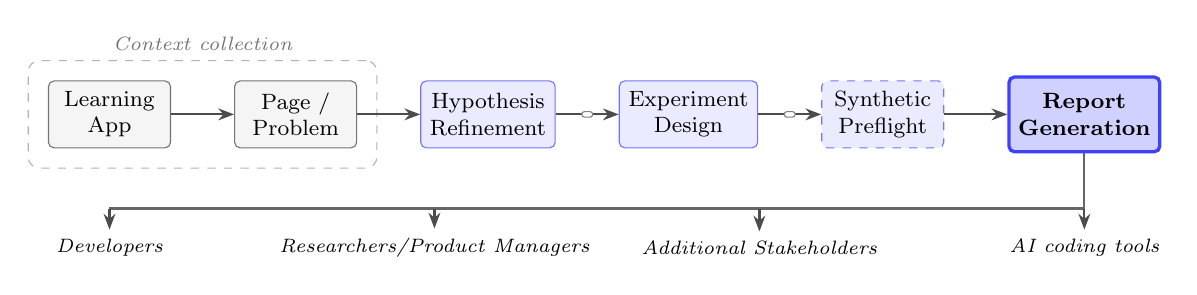
\begin{tikzpicture}[
  >={Stealth[length=2mm]},
  font=\footnotesize,
  phase/.style={
    draw=black!55, rounded corners=2pt,
    minimum width=1.55cm, minimum height=0.85cm,
    align=center, fill=gray!8
  },
  value/.style={
    draw=blue!55, rounded corners=2pt,
    minimum width=1.55cm, minimum height=0.85cm,
    align=center, fill=blue!8
  },
  optional/.style={
    draw=blue!55, dashed, rounded corners=2pt,
    minimum width=1.55cm, minimum height=0.85cm,
    align=center, fill=blue!8
  },
  report/.style={
    draw=blue!75, very thick, rounded corners=2pt,
    minimum width=1.65cm, minimum height=0.95cm,
    align=center, font=\footnotesize\bfseries,
    fill=blue!18
  },
  consumer/.style={font=\scriptsize\itshape, align=center},
  arr/.style={->, thick, draw=black!70},
  connect/.style={draw=black!60, thick},
  approval/.style={font=\scriptsize, fill=white, draw=black!50,
                   rounded corners=1pt, inner xsep=2pt, inner ysep=1pt}
]

% --- pipeline (left to right) ---
\node[phase] (app) at (0,0) {Learning\\App};
\node[phase, right=8mm of app]    (target) {Page /\\Problem};
\node[value, right=8mm of target] (idea)   {Hypothesis\\Refinement};
\node[value, right=8mm of idea]   (design) {Experiment\\Design};
\node[optional, right=8mm of design] (sim) {Synthetic\\Preflight};
\node[report, right=8mm of sim]   (report) {Report\\Generation};

\foreach \a/\b in {app/target, target/idea, idea/design, design/sim, sim/report} {
  \draw[arr] (\a) -- (\b);
}

% --- approval gates ---
\node[approval] at ($(idea.east)!0.5!(design.west)$) {\checkmark};
\node[approval] at ($(design.east)!0.5!(sim.west)$) {\checkmark};

% --- "Context collection" group around app + target ---
\begin{scope}[on background layer]
  \node[draw=black!30, dashed, rounded corners,
        fit=(app)(target), inner sep=2.5mm,
        label={[font=\scriptsize\itshape, black!55]above:Context collection}] {};
\end{scope}

% --- consumer fan-out below the report (evenly spaced across pipeline width) ---
\coordinate (cy) at ([yshift=-12mm]report.south);
\node[consumer] (res)   at (cy -| app)               {Developers};
\node[consumer] (ai)    at (cy -| report)            {AI coding tools};
\node[consumer] (dev)   at ($(res)!1/3!(ai)$)        {Researchers/Product Managers};
\node[consumer] (stake) at ($(res)!2/3!(ai)$)        {Additional Stakeholders};

\coordinate (bus) at ([yshift=-7mm]report.south);
\draw[connect] (report.south) -- (bus -| report);
\draw[connect] (bus -| res) -- (bus -| ai);
\foreach \t in {res, dev, stake, ai} {
  \draw[arr] (bus -| \t) -- (\t);
}
\end{tikzpicture}
\caption{Six-phase consulting workflow and report handoff. Context phases (dashed group, left) feed the AI-driven core; explicit user approvals (\checkmark) gate the major transitions, and the dashed Synthetic Preflight node is optional. The resulting report is the shared handoff artifact across researchers, developers, stakeholders, and/or AI coding tools.}

\Description{Horizontal pipeline of six phases connected by arrows: Learning App, Page / Problem (both grouped under a dashed Context-collection label), Hypothesis Refinement, Experiment Design, Synthetic Preflight (dashed border, indicating optional), and Report Generation (drawn with a heavier border as the central artifact). Small boxed checkmarks sit on the arrows between Hypothesis Refinement and Experiment Design, and between Experiment Design and Synthetic Preflight, indicating user-approval gates. Below the Report Generation box, four arrows fan out via a horizontal bus to four italicized labels: Developers, Researchers/Product Managers, Additional Stakeholders, and AI coding tools.}
\label{fig:workflow}
\end{figure}

\section{Consulting Workflow}

The flow has six phases, presented above in five grouped subsections. Context collection comes first; the later phases --- hypothesis refinement, experiment design, synthetic preflight, and report generation --- show how each step builds from initial information-gathering toward an implementation-ready experiment plan for UpGrade. We describe each phase in detail below.

\subsection{Context Collection}

The conversation opens by collecting basic context about the EdTech application and how it works: what the application does, who its learners are, the domain, and a description of the typical user flow. It then turns to the specific page, problem, or interaction where an experiment might run, including whether the user is trying to solve a problem, develop an intervention, or create a feature. Users can upload files such as screenshots or documents to help the AI provide more specific follow-up questions and suggestions.

\subsection{Ideation and Hypothesis Refinement}

This is the most dynamic phase. The user may arrive with a clear idea (``test whether adding a hint improves correctness rates''), an unfocused problem to solve (``students get stuck here''), or need more directed guidance on idea generation. The AI helps to refine ideas when needed, then proposes candidate interventions, providing comparison between alternative approaches if desired. During this phase, the system suggests outcome metrics based on contextual information gathered in the previous phase, then refines the approved approaches into a testable hypothesis, a sort of lightweight version of the \emph{iterative hypothesis generation, evaluation, and refinement} pattern in the AI co-scientist model~\cite{ai-coscientist}. After a hypothesis is approved, the consultant offers an optional related-paper search; when the user opts in, it summarizes up to three relevant papers and possible design implications, and the selected grounding can be included in the final report.

\subsection{UpGrade Experiment Design}

Once a hypothesis is approved, the AI assembles a concrete experiment design ready to run in UpGrade with all relevant parameters: name, description, app context, decision point, conditions with their assignment weights, and metrics. The user can ask questions, request alternatives, or edit any field before approving; only the participants setting is fixed (to \emph{Include All}) in the MVP.

\subsection{Synthetic Preflight Simulation}

With an approved design, the AI offers an optional synthetic preflight simulation against the hosted UpGrade demo backend, summarizing enrollment per condition, condition-level metric values, and basic interpretation cues. We make the caveat explicit: this is a \emph{preflight demonstration of UpGrade mechanics}, not evidence of the intervention's effect on learning outcomes. Rather, its purpose is to help users build familiarity with UpGrade concepts and output patterns, such as enrollment by condition and metric summaries, before running a real experiment; more experienced users may choose to skip this optional step.

\subsection{Report Generation}

In the final phase, the AI assembles a detailed markdown report covering the learning app description and other relevant context, a refined hypothesis, related research grounding (if used), proposed UpGrade experiment design, simulation summary (if used), a recommended implementation order, and templated setup and client-integration guidance with code examples. The report represents the primary handoff artifact across user roles and AI tools (if used). 

\section{Representative Use Case and Demo}

To make the workflow concrete, we walk through a fictional but representative scenario.

\textbf{Scenario.} \emph{ExampleMathApp} is a math learning application for middle-school students. On one of the problem pages for a particular topic, the product team has noticed that many students get this problem incorrect on the first try. They want to test whether adding an optional hint button would improve correctness rates on the first attempt.

\textbf{Walkthrough.} After describing the app (including a screenshot of the problem page), the primary concern, and the targeted student population, the user works with the AI to develop and refine a hypothesis: \emph{``Adding an optional hint button on this problem page will increase the correctness rate at first attempt without substantially increasing time-on-task.''} The AI proposes correctness rate and time-on-task as metrics. The consultant also offers the optional related-paper search described above; in this walkthrough, we skip that branch and proceed directly to the UpGrade design. Once the user approves, it produces the experiment design in Figure~\ref{fig:design}.

\begin{figure}[t]
\begin{verbatim}
Name:        Hint Button Experiment
Description: Tests whether adding an optional hint button
             improves correctness at first attempt on a target math problem.
App Context: example-math-app
Decision Point:
  Site:   problem_page
  Target: problem_123_hint_support
Conditions:
  control:     50%
  hint_button: 50%
Participants: Include All
Metrics:
  correctnessRate: Percent = CORRECT
  timeOnTask:     Mean
\end{verbatim}
\caption{Proposed UpGrade experiment design generated by the AI consultant for the ExampleMathApp hint-button scenario and included in the final report.}
\Description{A code-style listing showing the proposed UpGrade experiment configuration: name, description, app context, decision point (site and target), two conditions split 50/50, participants set to Include All, and two metrics (correctness rate and time on task).}
\label{fig:design}
\end{figure}

A synthetic simulation with 200 participants returns balanced enrollment (control 97, hint\_button 103), correctnessRate 78.4 for control vs.\ 84.5 for hint\_button, and timeOnTask 11.2 vs.\ 12.6. The simulation suggests that \emph{hint\_button} trends higher on correctness in this synthetic run, but notes that this is not meant to replace a true randomized experiment. The final report bundles the app and page descriptions, hypothesis, UpGrade experiment design, simulation summary with caveat, recommended implementation order, setup and experiment-creation guidance, and client-integration code examples.

The generated markdown report is the prototype's central artifact, making the experiment plan shareable across researchers, developers, and other stakeholders. As input to AI coding tools, the report can be used within the client application to support adding UpGrade API calls, implementing intervention variations in the client app, or other actions.

\section{Discussion, Limitations, and Future Vision}

The prototype described here occupies an intentionally narrow space in comparison to recent AI-assisted research tools. The AI co-scientist~\cite{ai-coscientist} uses tournament-style generation, debate, and evolution to autonomously traverse large, open-ended hypothesis spaces in domains like drug repurposing, while the AI Scientist~\cite{end-to-end-ai-research} goes further toward end-to-end automation, from ideation through manuscript generation. While our tool borrows the high-level \emph{iterative hypothesis generation, evaluation, and refinement} pattern from these approaches, we apply it to the tightly scoped challenge of translating an EdTech team's product or research idea into a concrete UpGrade experiment design. Where other systems maximize autonomous exploration, this AI consultant maximizes human control, ensuring that every major phase transition relies on explicit user approval, more appropriate for users who require strong control over interventions and interpretability of outcomes.

\textbf{Limitations.} The MVP currently supports only simple randomized between-subjects designs with individual-level assignment and a single decision point. This is a deliberate scoping choice for the prototype rather than a constraint of UpGrade itself, and relaxing the single-decision-point restriction to support richer designs is the first limitation we plan to address. The synthetic preflight demonstrates UpGrade mechanics rather than learning outcomes and should not substitute for a properly powered randomized trial. Finally, the prototype has not yet been evaluated with real EdTech teams; the walkthrough in Section 5 is illustrative of a commonly encountered scenario. We anticipate being able to evaluate this tool during upcoming platform onboarding in Fall 2026. 

\textbf{Future vision.} Looking ahead, in addition to supporting more complex experimental designs, the report could evolve into the hub of a human-supervised pipeline~\cite{end-to-end-ai-research, asi-evolve}: a researcher approves the report; an AI coding agent drafts the variant's pull request for a developer to review and merge; automated tooling provisions the UpGrade experiment for the researcher to verify and launch; and AI-assisted analysis informs the next planning cycle. Each transition preserves human review, keeping the artifact a semi-executable specification rather than an autonomous workflow. In the near term, we will demonstrate the prototype at the workshop and pilot it with external EdTech teams during UpGrade onboarding.

\bibliographystyle{ACM-Reference-Format}
\bibliography{references}

\end{document}
